% =============================================================
% Capitolo: Framework di Valutazione — NLU Accuracy e Agent Routing
% Progetto: MCP_ECOM — Agente e-commerce basato su MCP
% =============================================================

\chapter{Framework di Valutazione: NLU Accuracy e Agent Routing}
\label{chap:evaluation}

% ─────────────────────────────────────────────────────────────
\section{Motivazione e Obiettivi}
\label{sec:eval-intro}
% ─────────────────────────────────────────────────────────────

Un agente conversazionale per l'e-commerce opera su due piani distinti:
il piano \emph{semantico}, dove comprende l'intenzione dell'utente ed
estrae le informazioni strutturate dalla query in linguaggio naturale, e
il piano \emph{decisionale}, dove seleziona la sequenza corretta di tool
MCP da invocare. Errori nel primo piano si propagano inevitabilmente al
secondo: un parser che non riconosce il vincolo di prezzo non può
produrre una chiamata corretta a \texttt{search\_products}.

Per misurare la qualità di entrambi i piani in modo sistematico e
riproducibile, è stata progettata ed implementata un'infrastruttura di
test dedicata all'interno della cartella \texttt{tests/eval/}. Il
framework è composto da tre componenti principali:

\begin{enumerate}
    \item \textbf{Dataset ground-truth} (\texttt{intent\_dataset.json}) —
          un corpus annotato di 30 query utente in italiano con le
          estrazioni semantiche attese, allineato allo schema Pydantic
          reale del parser LLM.
    \item \textbf{Test runner NLU} (\texttt{test\_intent\_accuracy.py}) —
          un valutatore asincrono che calcola metriche di precisione a
          tre livelli strutturali sulla risposta del parser.
    \item \textbf{Test di routing agente} (\texttt{test\_agent\_routing.py}) —
          una suite pytest che verifica il comportamento deterministico
          del planner \texttt{ReactPlanner} senza dipendenze esterne.
\end{enumerate}

Il framework include inoltre \texttt{eval\_metrics.py}, che fornisce
implementazioni pure di \textbf{MRR} (\emph{Mean Reciprocal Rank}) e
\textbf{nDCG@K} (\emph{Normalized Discounted Cumulative Gain}), pronte
per essere integrate in futuri benchmark del layer RAG.

% ─────────────────────────────────────────────────────────────
\section{Dataset Ground-Truth}
\label{sec:eval-dataset}
% ─────────────────────────────────────────────────────────────

\subsection{Problema dello Schema Disallineato}
\label{subsec:schema-drift}

La versione iniziale del dataset conteneva cinque entry con un formato
\emph{piatto} non conforme all'output reale del parser:

\begin{lstlisting}[language=json, caption={Formato obsoleto del dataset (pre-refactoring)}]
{
  "id": 1,
  "query": "Vorrei un iPhone rigenerato blu sotto i 300 euro",
  "expected": {
    "brand": "Apple",
    "condition": "ricondizionato",
    "max_price": 300.0
  }
}
\end{lstlisting}

Il modulo \texttt{app/services/parser.py} produce invece un output
strutturato con campi annidati: \texttt{brands} è una lista, la
condizione e il prezzo sono elementi di un array \texttt{constraints}
con tipo, operatore e valore separati. Questo disallineamento rendeva
il confronto nel test runner sistematicamente errato, portando a
metriche di precisione artificialmente basse e al silenzioso abbandono
di tutti i constraint estratti.

\subsection{Schema Corretto}
\label{subsec:correct-schema}

Il dataset è stato interamente riscritto per conformarsi allo schema
\texttt{DEFAULT\_RESULT\_TEMPLATE} definito in \texttt{parser.py}:

\begin{lstlisting}[language=json, caption={Formato corretto del dataset, allineato al parser LLM}]
{
  "id": 1,
  "query": "Vorrei un iPhone rigenerato blu che stia sotto i 300 euro.
            Ma cercalo venduto da pegaso_italia per favore.",
  "expected": {
    "product": "iPhone",
    "brands": ["Apple"],
    "constraints": [
      {"type": "condition", "value": "refurbished"},
      {"type": "price", "operator": "<=", "value": 300},
      {"type": "aspect", "name": "color", "value": "blue"}
    ],
    "target_seller": "pegaso_italia"
  }
}
\end{lstlisting}

I campi testabili per ogni entry sono:

\begin{table}[htbp]
\centering
\caption{Campi del dataset e relativi tipi di confronto}
\label{tab:dataset-fields}
\begin{tabular}{lll}
\toprule
\textbf{Campo} & \textbf{Tipo} & \textbf{Metrica} \\
\midrule
\texttt{product}       & stringa scalare   & Exact match (normalizzato) \\
\texttt{product\_type} & enum              & Exact match \\
\texttt{target\_seller}& stringa scalare   & Exact match \\
\texttt{brands}        & lista di stringhe & Precision/Recall su set \\
\texttt{exclusions}    & lista di stringhe & Precision/Recall su set \\
\texttt{constraints}   & lista di oggetti  & Match per tipo con tolleranza \\
\bottomrule
\end{tabular}
\end{table}

\subsection{Copertura del Dataset}
\label{subsec:dataset-coverage}

Il dataset è stato espanso da 5 a \textbf{30 entry}, coprendo
sistematicamente le seguenti categorie di query:

\begin{table}[htbp]
\centering
\caption{Categorie di query coperte dal dataset}
\label{tab:dataset-coverage}
\begin{tabular}{lp{7cm}}
\toprule
\textbf{Categoria} & \textbf{Esempio / Caratteristica} \\
\midrule
Query base con brand     & \textit{``Cerco scarpe Nike da corsa''} \\
Prezzo massimo (\texttt{<=})   & \textit{``PS5 usata a meno di 400€''} \\
Prezzo minimo (\texttt{>=})    & \textit{``Mouse gaming sopra i 50 euro''} \\
Range di prezzo          & \textit{``Smartwatch tra i 200 e i 500 euro''} \\
Condizione esplicita     & \textit{``Solo nuovo / usato / ricondizionato''} \\
Seller specifico         & \textit{``Da venditore apple\_store\_it''} \\
Multi-brand              & \textit{``iPhone o Samsung Galaxy nuovo''} \\
Aspect constraint        & Colore, storage, taglia, piattaforma \\
Esclusioni               & \textit{``che non sia ricondizionato''} \\
Accessori / Parti        & \texttt{product\_type: Accessory | Part} \\
Query brevi              & \textit{``Samsung usato''}, \textit{``iPhone''} \\
Query con rumore sintattico & \textit{``vorrei tipo cercare un telefono mm...''} \\
Query complesse combinate & Più constraint + seller + brand insieme \\
\bottomrule
\end{tabular}
\end{table}

% ─────────────────────────────────────────────────────────────
\section{Test Runner NLU: Valutazione Multi-Livello}
\label{sec:eval-nlu-runner}
% ─────────────────────────────────────────────────────────────

\subsection{Problema della Funzione di Confronto Originale}
\label{subsec:f1-original}

La funzione \texttt{compute\_f1\_for\_dict} originale eseguiva un
appiattimento (\emph{flattening}) del dizionario predetto e ignorava
esplicitamente i blocchi \texttt{constraints}, \texttt{preferences} e
\texttt{compatibilities}:

\begin{lstlisting}[language=Python, caption={Chiavi ignorate nel confronto originale}]
ignore_keys = [
    "original_query", "confidence",
    "constraints", "preferences",      # <- ignorati completamente
    "compatibilities", "target_seller"
]
\end{lstlisting}

Il risultato era che le metriche di precision/recall non includevano
mai i confronti su prezzo e condizione — le dimensioni più
critiche dell'estrazione semantica.

\subsection{Architettura del Confronto Multi-Livello}
\label{subsec:multilevel-compare}

La funzione di confronto è stata sostituita con \texttt{compare\_parser\_output},
che opera su tre livelli strutturali distinti:

\begin{figure}[htbp]
    \centering
    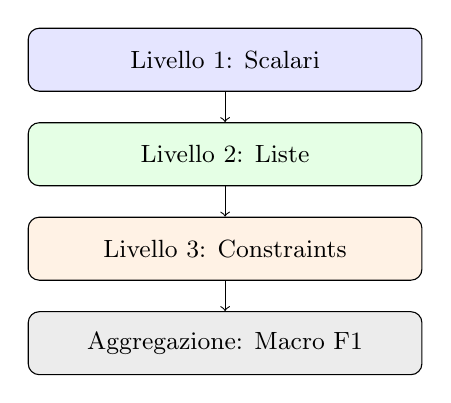
\begin{tikzpicture}[
        node distance=1.2cm,
        box/.style={rectangle, draw, rounded corners, minimum width=5cm,
                    minimum height=0.8cm, font=\small}
    ]
        \node[box, fill=blue!10]  (l1) {Livello 1: Scalari};
        \node[box, fill=green!10, below of=l1] (l2) {Livello 2: Liste};
        \node[box, fill=orange!10, below of=l2] (l3) {Livello 3: Constraints};
        \node[box, fill=gray!15, below of=l3] (agg) {Aggregazione: Macro F1};

        \draw[->] (l1) -- (l2);
        \draw[->] (l2) -- (l3);
        \draw[->] (l3) -- (agg);
    \end{tikzpicture}
    \caption{Architettura del confronto multi-livello in \texttt{compare\_parser\_output}}
    \label{fig:multilevel-compare}
\end{figure}

\paragraph{Livello 1 — Scalari.}
I campi \texttt{product}, \texttt{target\_seller} e \texttt{product\_type}
vengono confrontati con exact match dopo normalizzazione (lowercase + strip).
Ogni campo contribuisce con un punteggio binario $\{0, 1\}$.

\paragraph{Livello 2 — Liste.}
I campi \texttt{brands} e \texttt{exclusions} vengono convertiti in
insiemi normalizzati e confrontati con \emph{set intersection}. Per
ciascun campo si calcolano precision e recall:

\[
\text{Precision} = \frac{|P \cap E|}{|P|}, \quad
\text{Recall}    = \frac{|P \cap E|}{|E|}
\]

dove $P$ è l'insieme dei valori predetti ed $E$ quello atteso. L'F1
del singolo campo è la media armonica delle due.

\paragraph{Livello 3 — Constraints.}
I constraint vengono raggruppati per \texttt{type}. Per ogni constraint
atteso si cerca una corrispondenza tra quelli predetti dello stesso tipo.
Il confronto è adattato al tipo semantico:

\begin{itemize}
    \item \textbf{price}: matching su operatore (upper/lower bound) e
          valore con tolleranza del $5\%$; il tipo \texttt{between}
          richiede la corrispondenza di entrambi gli estremi.
    \item \textbf{condition}: exact match sul valore normalizzato
          (\texttt{new}, \texttt{used}, \texttt{refurbished}).
    \item \textbf{aspect}: double match su \texttt{name} e \texttt{value}
          (es.\ \texttt{color: blue}, \texttt{storage: 128GB}).
\end{itemize}

\begin{lstlisting}[language=Python, caption={Logica di matching per constraint di tipo prezzo}]
if ctype == "price":
    upper_ops = {"<=", "<"}
    lower_ops = {">=", ">"}
    if exp_op in upper_ops and pred_op in upper_ops:
        if abs(pred_val - exp_val) / max(exp_val, 1) <= 0.05:
            return True
    elif exp_op == "between" and pred_op == "between":
        lo_ok = abs(pred_val[0] - exp_val[0]) / max(exp_val[0], 1) <= 0.05
        hi_ok = abs(pred_val[1] - exp_val[1]) / max(exp_val[1], 1) <= 0.05
        if lo_ok and hi_ok:
            return True
\end{lstlisting}

\subsection{Report di Output}
\label{subsec:eval-output}

Il runner produce per ogni query un report strutturato e, al termine,
le metriche aggregate sull'intero dataset:

\begin{lstlisting}[caption={Esempio di output del test runner}]
[ID 1] Query: 'Vorrei un iPhone rigenerato blu...'
  SCALAR     : {'product': True, 'target_seller': True}
  LISTS      : {'brands': {'precision': 1.0, 'recall': 1.0, 'f1': 1.0}}
  CONSTRAINTS: {'condition': True, 'price:<=': True, 'aspect:color': True}
  AGGREGATE  : scalar_acc=1.0  list_f1=1.0  constraint_acc=1.0  macro_f1=1.0

====================================
  RISULTATI FINALI SU 30 QUERY:
  Mean Macro F1   : 0.XXX
  Exact Matches   : X/30 (X.X%)
====================================
\end{lstlisting}

Il test runner si lancia direttamente come script Python (senza pytest,
poiché richiede chiamate asincrone al parser LLM) e carica
automaticamente le variabili d'ambiente dal file \texttt{.env}:

\begin{lstlisting}[language=bash, caption={Comando di esecuzione del test runner NLU}]
python tests/eval/test_intent_accuracy.py
\end{lstlisting}

% ─────────────────────────────────────────────────────────────
\section{Test di Routing del Planner}
\label{sec:eval-routing}
% ─────────────────────────────────────────────────────────────

\subsection{Obiettivo e Approccio}
\label{subsec:routing-objective}

La correttezza del routing deterministico del \texttt{ReactPlanner}
viene verificata da \texttt{test\_agent\_routing.py}, una suite pytest
completamente \emph{offline}: non richiede il server MCP, Redis, il
database né l'LLM. Testa i metodi privati del planner in isolamento
tramite un oggetto \texttt{MockMemory} minimale:

\begin{lstlisting}[language=Python, caption={Stub MockMemory usato nei test di routing}]
class MockMemory:
    def __init__(self, query: str, mcp_mode: str = "standard",
                 has_explicit_id: bool = False):
        self.user_query = query
        self.mcp_mode = mcp_mode
        self.last_seller_name = None
        self.detected_intent = None
        if has_explicit_id:
            self.user_query = query + " 123456789012"
\end{lstlisting}

\subsection{Test di \texttt{\_infer\_intent}}
\label{subsec:test-infer-intent}

Il metodo \texttt{\_infer\_intent} implementa un routing euristico
basato su keyword matching. Il test parametrizzato copre 19 casi:

\begin{table}[htbp]
\centering
\caption{Casi di test per \texttt{\_infer\_intent} (selezione)}
\label{tab:infer-intent-cases}
\begin{tabular}{lll}
\toprule
\textbf{Query} & \textbf{Intent atteso} & \textbf{Trigger} \\
\midrule
\textit{cerca iPhone 13 ricondizionato}      & \texttt{product\_search}  & default \\
\textit{feedback del venditore pegaso\_it}   & \texttt{seller\_analysis} & keyword: \textit{feedback} \\
\textit{confronta iPhone 14 e Samsung S23}   & \texttt{comparison}       & keyword: \textit{confronta} \\
\textit{quanto costa spedire questo articolo}& \texttt{shipping}         & keyword: \textit{costa spedire} \\
\textit{contatta il negozio per me}          & \texttt{contact\_seller}  & keyword: \textit{contatta} \\
\textit{andamento prezzi smartphone}         & \texttt{market\_trends}   & keyword: \textit{andamento + prezz} \\
\textit{statistiche mercato tech}            & \texttt{market\_trends}   & keyword: \textit{statistiche} \\
\textit{ciao}                                & \texttt{conversation}     & greeting \\
\textit{(stringa vuota)}                     & \texttt{conversation}     & guard clause \\
\bottomrule
\end{tabular}
\end{table}

Un caso di interesse emerso durante lo sviluppo dei test riguarda la
\textbf{precedenza delle keyword}: la query
\textit{``contatta il venditore''} viene classificata come
\texttt{seller\_analysis} anziché \texttt{contact\_seller}, perché il
controllo sulla parola \texttt{venditore} precede quello su
\texttt{contatta} nel codice del planner. I test documentano questo
comportamento come comportamento atteso, garantendo che future
modifiche al planner non alterino la precedenza silenziosamente.

\subsection{Test di \texttt{\_ordered\_tools\_for\_intent}}
\label{subsec:test-tool-order}

Per ogni intent viene verificato il primo tool nella sequenza restituita
da \texttt{\_ordered\_tools\_for\_intent}, e in alcuni casi l'intera
sequenza:

\begin{lstlisting}[language=Python, caption={Esempio di test sul tool ordering}]
def test_item_details_with_explicit_id():
    """Con un ID eBay nella query, item_details usa get_item_details direttamente."""
    planner = ReactPlanner(llm_engine="rule_based")
    memory = MockMemory("dettagli articolo", has_explicit_id=True)
    tools = planner._ordered_tools_for_intent("item_details", memory)
    assert tools == ["get_item_details"]

def test_item_details_without_explicit_id():
    """Senza ID, item_details inizia con search_products per trovare l'articolo."""
    planner = ReactPlanner(llm_engine="rule_based")
    memory = MockMemory("voglio dettagli su questo prodotto")
    tools = planner._ordered_tools_for_intent("item_details", memory)
    assert tools[0] == "search_products"
    assert "get_item_details" in tools
\end{lstlisting}

Sono inclusi test per casi speciali: modalità Playwright (che instrada
\texttt{product\_search} su \texttt{browser\_navigate}), wishlist con
ID esplicito (che salta il passo di ricerca), e budget dei tool (che
impedisce la ri-esecuzione di un tool oltre il limite impostato.

\subsection{Test di Completezza degli Intent}
\label{subsec:test-completeness}

Un test di completezza verifica che ogni intent definito in
\texttt{VALID\_INTENTS} — esclusi \texttt{conversation} e
\texttt{playwright\_search} — restituisca almeno un tool dalla funzione
di routing:

\begin{lstlisting}[language=Python, caption={Test di completezza del mapping intent→tool}]
def test_all_valid_intents_have_tool_mapping():
    from app.agent.planner import VALID_INTENTS
    planner = ReactPlanner(llm_engine="rule_based")
    memory = MockMemory("test query")
    skip = {"conversation", "playwright_search"}
    for intent in VALID_INTENTS - skip:
        tools = planner._ordered_tools_for_intent(intent, memory)
        assert len(tools) > 0, f"Intent '{intent}' returned no tools"
\end{lstlisting}

Questo test funge da \emph{regression guard}: se in futuro viene
aggiunto un nuovo intent a \texttt{VALID\_INTENTS} senza aggiornare
la funzione di routing, il test fallirà immediatamente.

\subsection{Risultati della Suite}
\label{subsec:routing-results}

La suite conta \textbf{35 test}, tutti eseguiti in modalità offline.
Il tempo di esecuzione è di circa 2 secondi sull'hardware di sviluppo:

\begin{lstlisting}[language=bash, caption={Esecuzione e output della suite di routing}]
pytest tests/eval/test_agent_routing.py -v
# ...
# 35 passed in 2.27s
\end{lstlisting}

% ─────────────────────────────────────────────────────────────
\section{Metriche RAG: MRR e nDCG}
\label{sec:eval-rag-metrics}
% ─────────────────────────────────────────────────────────────

Il file \texttt{eval\_metrics.py} implementa due funzioni di valutazione
per il layer di retrieval semantico (\texttt{app/services/rag/}), pronte
per l'integrazione in futuri benchmark end-to-end.

\subsection{Mean Reciprocal Rank (MRR)}
\label{subsec:mrr}

L'MRR misura quanto in alto nella lista dei risultati compare il primo
item rilevante. Per un batch di query:

\[
\text{MRR} = \frac{1}{|Q|} \sum_{i=1}^{|Q|} \frac{1}{\text{rank}_i}
\]

dove $\text{rank}_i$ è la posizione (1-based) del primo item rilevante
nella lista restituita per la query $i$. Un valore di $\text{MRR} = 1.0$
indica che il risultato corretto è sempre in prima posizione.

\begin{lstlisting}[language=Python, caption={Implementazione MRR in \texttt{eval\_metrics.py}}]
def mean_reciprocal_rank(
    retrieved_lists: List[List[str]],
    relevant_items: List[str]
) -> float:
    mrr_sum = 0.0
    for r_list, rel_item in zip(retrieved_lists, relevant_items):
        try:
            rank = r_list.index(rel_item) + 1   # 1-based
            mrr_sum += 1.0 / rank
        except ValueError:
            mrr_sum += 0.0                       # item non trovato
    return mrr_sum / len(retrieved_lists)
\end{lstlisting}

\subsection{Normalized Discounted Cumulative Gain (nDCG@K)}
\label{subsec:ndcg}

L'nDCG@K valuta la qualità dell'ordinamento dei primi $K$ risultati
rispetto a un ordinamento ideale, pesando la rilevanza con un fattore
logaritmico decrescente basato sulla posizione:

\[
\text{DCG@K} = \sum_{i=1}^{K} \frac{\text{rel}_i}{\log_2(i+1)}, \quad
\text{nDCG@K} = \frac{\text{DCG@K}}{\text{IDCG@K}}
\]

dove IDCG@K è il DCG calcolato sull'ordinamento ideale (risultati
ordinati per rilevanza decrescente). Il punteggio nDCG è normalizzato
in $[0, 1]$.

Nel contesto del sistema MCP\_ECOM, il punteggio di rilevanza di ogni
prodotto può essere il \texttt{combined\_score} calcolato dalla
pipeline LTR (\emph{Learning to Rank}) di \texttt{search\_pipeline.py},
che combina similarità semantica, trust score del venditore, sentiment
e deviazione di prezzo.

% ─────────────────────────────────────────────────────────────
\section{Struttura della Cartella \texttt{tests/eval}}
\label{sec:eval-structure}
% ─────────────────────────────────────────────────────────────

\begin{table}[htbp]
\centering
\caption{File del framework di valutazione}
\label{tab:eval-files}
\begin{tabular}{lp{8cm}}
\toprule
\textbf{File} & \textbf{Ruolo} \\
\midrule
\texttt{intent\_dataset.json}      & Dataset ground-truth con 30 query annotate
                                     (schema allineato al parser LLM) \\
\texttt{test\_intent\_accuracy.py} & Runner asincrono per valutazione NLU;
                                     produce metriche F1 a tre livelli \\
\texttt{test\_agent\_routing.py}   & Suite pytest offline (35 test) per
                                     il routing deterministico del planner \\
\texttt{eval\_metrics.py}          & Implementazioni pure di MRR e nDCG@K
                                     per future valutazioni del layer RAG \\
\bottomrule
\end{tabular}
\end{table}

\begin{lstlisting}[language=bash, caption={Comandi di esecuzione del framework di valutazione}]
# Valutazione NLU accuracy (richiede LLM attivo)
python tests/eval/test_intent_accuracy.py

# Test di routing (offline, nessuna dipendenza esterna)
pytest tests/eval/test_agent_routing.py -v

# Intera suite eval
pytest tests/eval/ -v --tb=short
\end{lstlisting}

% ─────────────────────────────────────────────────────────────
\section{Riepilogo}
\label{sec:eval-summary}
% ─────────────────────────────────────────────────────────────

Il framework di valutazione di MCP\_ECOM copre sistematicamente i due
livelli critici dell'agente: la comprensione linguistica e il routing
decisionale.

\begin{table}[htbp]
\centering
\caption{Proprietà architetturali del framework di valutazione}
\label{tab:eval-summary}
\begin{tabular}{lll}
\toprule
\textbf{Componente} & \textbf{Proprietà} & \textbf{Valore} \\
\midrule
Dataset NLU        & Entry totali              & 30 query annotate \\
Dataset NLU        & Schema                    & Allineato a \texttt{DEFAULT\_RESULT\_TEMPLATE} \\
Test NLU           & Livelli di confronto      & 3 (scalari, liste, constraints) \\
Test NLU           & Tolleranza prezzo         & $\pm 5\%$ sul valore numerico \\
Test routing       & Test totali               & 35 \\
Test routing       & Dipendenze esterne        & Nessuna (completamente offline) \\
Test routing       & Tempo di esecuzione       & $\approx 2$ secondi \\
Metriche RAG       & Algoritmi disponibili     & MRR, nDCG@K \\
\bottomrule
\end{tabular}
\end{table}

La separazione tra i test NLU (asincroni, richiedono il parser LLM)
e i test di routing (sincroni, completamente offline) consente di
eseguire la validazione del planner in ogni ambiente CI senza dipendenze
da servizi esterni, mentre i test NLU vengono riservati alle fasi di
integrazione dove il modello LLM è disponibile.
